% Pivot decomposition figure: G on 43 vertices next to the same graph
% redrawn around the pivot v with neighborhood A and anti-neighborhood B.
% Included from main.tex via % Pivot decomposition figure: G on 43 vertices next to the same graph
% redrawn around the pivot v with neighborhood A and anti-neighborhood B.
% Included from main.tex via % Pivot decomposition figure: G on 43 vertices next to the same graph
% redrawn around the pivot v with neighborhood A and anti-neighborhood B.
% Included from main.tex via % Pivot decomposition figure: G on 43 vertices next to the same graph
% redrawn around the pivot v with neighborhood A and anti-neighborhood B.
% Included from main.tex via \input{figures/pivot-decomposition}.

\begin{figure}[ht]
	\centering
	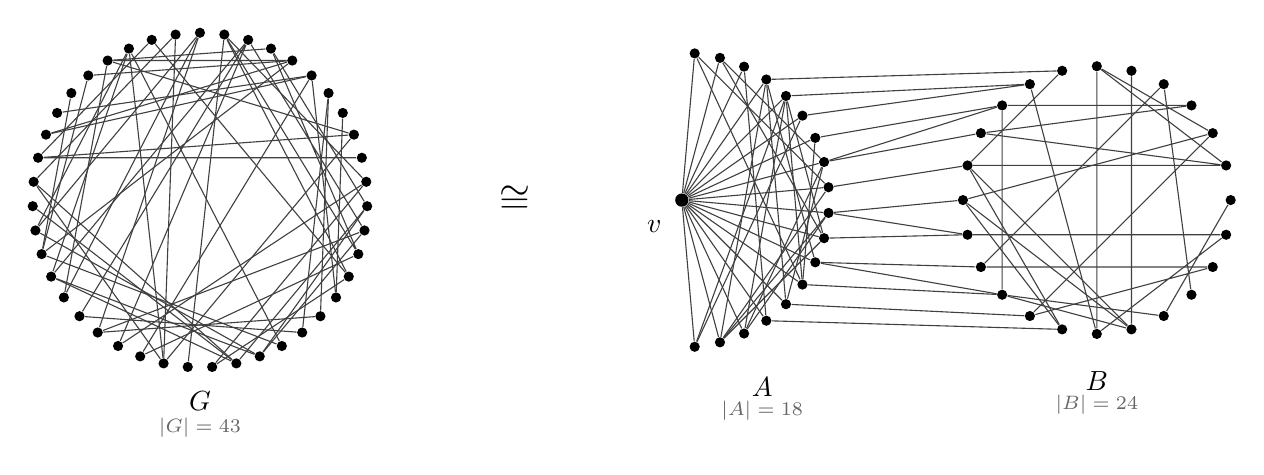
\begin{tikzpicture}[scale=0.85,
			vertex/.style={circle, fill, inner sep=1.3pt},
			pivot/.style={circle, fill, inner sep=1.7pt},
			e/.style={thin, black!75}
		]
		% Pivot vertex.
		\node[pivot, label={[label distance=1mm]below left:$v$}] (v) at (0,0) {};

		% Neighborhood A: 18 vertices, all adjacent to v.
		\foreach \i in {0,...,17} {
				\node[vertex] (a\i) at ({-85 + 10*\i}:2.2) {};
			}

		% Anti-neighborhood B: 24 vertices, none adjacent to v.
		\foreach \i [evaluate=\i as \bx using 6.2 + 2*cos(15*\i),
			evaluate=\i as \by using 2*sin(15*\i)] in {0,...,23} {
				\node[vertex] (b\i) at (\bx, \by) {};
			}

		% The whole graph G: 43 vertices on a circle.
		\foreach \i [evaluate=\i as \gx using -7.2 + 2.5*cos(90 + 8.372093*\i),
			evaluate=\i as \gy using 2.5*sin(90 + 8.372093*\i)] in {0,...,42} {
				\node[vertex] (g\i) at (\gx, \gy) {};
			}

		% Illustrative random edges inside G.
		\draw[e] (g13) -- (g39) (g16) -- (g41) (g18) -- (g41);
		\draw[e] (g1) -- (g10) (g32) -- (g40) (g10) -- (g23);
		\draw[e] (g3) -- (g25) (g9) -- (g34) (g29) -- (g42);
		\draw[e] (g18) -- (g33) (g19) -- (g38) (g0) -- (g12);
		\draw[e] (g20) -- (g35) (g33) -- (g42) (g1) -- (g20);
		\draw[e] (g30) -- (g40) (g30) -- (g42) (g31) -- (g41);
		\draw[e] (g0) -- (g17) (g21) -- (g42) (g7) -- (g38);
		\draw[e] (g14) -- (g24) (g8) -- (g39) (g5) -- (g13);
		\draw[e] (g4) -- (g39) (g22) -- (g33) (g0) -- (g15);
		\draw[e] (g24) -- (g32) (g10) -- (g20) (g3) -- (g20);
		\draw[e] (g14) -- (g23) (g19) -- (g30) (g3) -- (g12);
		\draw[e] (g12) -- (g24) (g17) -- (g27) (g28) -- (g38);
		\draw[e] (g17) -- (g31) (g4) -- (g40) (g3) -- (g14);
		\draw[e] (g13) -- (g25) (g4) -- (g15) (g9) -- (g35);
		\draw[e] (g8) -- (g38) (g23) -- (g32) (g24) -- (g31);
		\draw[e] (g5) -- (g39) (g6) -- (g13) (g27) -- (g37);
		\draw[e] (g22) -- (g29) (g14) -- (g41) (g11) -- (g23);
		\draw[e] (g16) -- (g26) (g2) -- (g29) (g2) -- (g9);
		\draw[e] (g28) -- (g36) (g26) -- (g37) (g4) -- (g35);

		% Edges from v into A.
		\foreach \i in {0,...,17} \draw[e] (v) -- (a\i);

		% Illustrative edges inside A.
		\draw[e] (a4) -- (a14) (a2) -- (a8) (a1) -- (a9);
		\draw[e] (a1) -- (a7) (a2) -- (a13) (a5) -- (a11);
		\draw[e] (a0) -- (a12) (a1) -- (a8) (a4) -- (a10);
		\draw[e] (a1) -- (a14) (a6) -- (a14) (a3) -- (a15);
		\draw[e] (a5) -- (a13) (a2) -- (a10) (a9) -- (a17);
		\draw[e] (a5) -- (a17) (a10) -- (a16) (a7) -- (a16);
		\draw[e] (a0) -- (a13) (a7) -- (a13);

		% Illustrative edges inside B.
		\draw[e] (b6) -- (b18) (b4) -- (b14) (b12) -- (b19);
		\draw[e] (b13) -- (b23) (b15) -- (b19) (b5) -- (b19);
		\draw[e] (b0) -- (b20) (b18) -- (b23) (b16) -- (b22);
		\draw[e] (b1) -- (b6) (b15) -- (b20) (b3) -- (b9);
		\draw[e] (b11) -- (b19) (b1) -- (b11) (b1) -- (b10);
		\draw[e] (b2) -- (b6) (b11) -- (b17) (b3) -- (b10);
		\draw[e] (b2) -- (b12) (b2) -- (b16) (b4) -- (b21);
		\draw[e] (b7) -- (b11) (b8) -- (b18) (b9) -- (b15);
		\draw[e] (b12) -- (b17) (b14) -- (b22);

		% Illustrative cross edges between A and B.
		\draw[e] (a8) -- (b12) (a9) -- (b11) (a7) -- (b13)
		(a10) -- (b10) (a6) -- (b14) (a11) -- (b9) (a5) -- (b15);
		\draw[e] (a3) -- (b17) (a4) -- (b16) (a6) -- (b15)
		(a8) -- (b13) (a10) -- (b9) (a12) -- (b8)
		(a13) -- (b8) (a14) -- (b7);

		% Isomorphism between the two depictions.
		\node[font=\Large] at (-2.5, 0) {$\cong$};

		% Group labels.
		\node at (-7.2, -3.0) {$G$};
		\node[font=\scriptsize, text=black!60] at (-7.2, -3.4) {$|G| = 43$};
		\node at (1.2, -2.8) {$A$};
		\node[font=\scriptsize, text=black!60] at (1.2, -3.15) {$|A| = 18$};
		\node at (6.2, -2.7) {$B$};
		\node[font=\scriptsize, text=black!60] at (6.2, -3.05) {$|B| = 24$};
	\end{tikzpicture}
	\caption{Illustrative decomposition into pivot $v$, neighborhood $A$ and anti-neighborhood $B$.}
\end{figure}
.

\begin{figure}[ht]
	\centering
	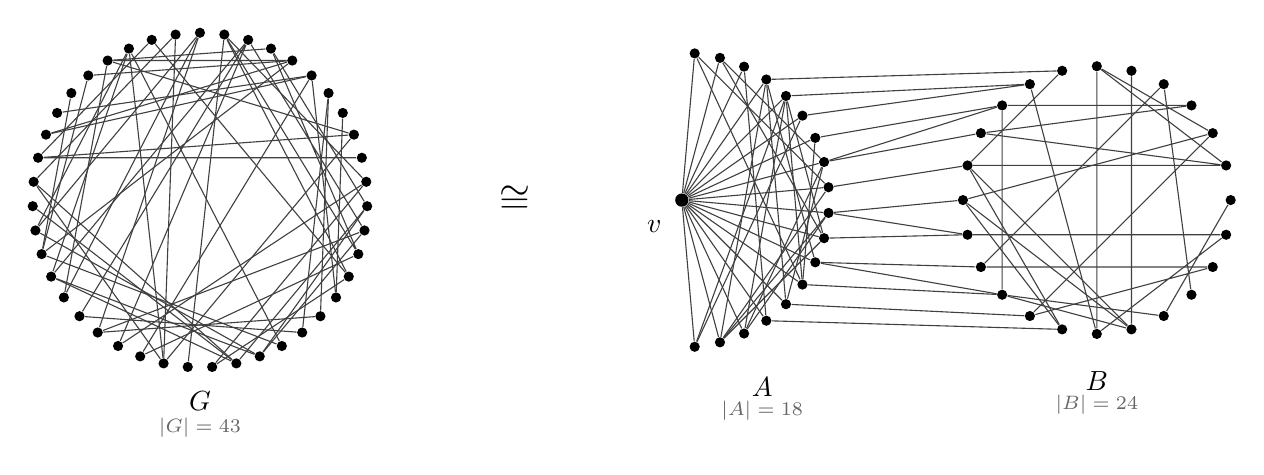
\begin{tikzpicture}[scale=0.85,
			vertex/.style={circle, fill, inner sep=1.3pt},
			pivot/.style={circle, fill, inner sep=1.7pt},
			e/.style={thin, black!75}
		]
		% Pivot vertex.
		\node[pivot, label={[label distance=1mm]below left:$v$}] (v) at (0,0) {};

		% Neighborhood A: 18 vertices, all adjacent to v.
		\foreach \i in {0,...,17} {
				\node[vertex] (a\i) at ({-85 + 10*\i}:2.2) {};
			}

		% Anti-neighborhood B: 24 vertices, none adjacent to v.
		\foreach \i [evaluate=\i as \bx using 6.2 + 2*cos(15*\i),
			evaluate=\i as \by using 2*sin(15*\i)] in {0,...,23} {
				\node[vertex] (b\i) at (\bx, \by) {};
			}

		% The whole graph G: 43 vertices on a circle.
		\foreach \i [evaluate=\i as \gx using -7.2 + 2.5*cos(90 + 8.372093*\i),
			evaluate=\i as \gy using 2.5*sin(90 + 8.372093*\i)] in {0,...,42} {
				\node[vertex] (g\i) at (\gx, \gy) {};
			}

		% Illustrative random edges inside G.
		\draw[e] (g13) -- (g39) (g16) -- (g41) (g18) -- (g41);
		\draw[e] (g1) -- (g10) (g32) -- (g40) (g10) -- (g23);
		\draw[e] (g3) -- (g25) (g9) -- (g34) (g29) -- (g42);
		\draw[e] (g18) -- (g33) (g19) -- (g38) (g0) -- (g12);
		\draw[e] (g20) -- (g35) (g33) -- (g42) (g1) -- (g20);
		\draw[e] (g30) -- (g40) (g30) -- (g42) (g31) -- (g41);
		\draw[e] (g0) -- (g17) (g21) -- (g42) (g7) -- (g38);
		\draw[e] (g14) -- (g24) (g8) -- (g39) (g5) -- (g13);
		\draw[e] (g4) -- (g39) (g22) -- (g33) (g0) -- (g15);
		\draw[e] (g24) -- (g32) (g10) -- (g20) (g3) -- (g20);
		\draw[e] (g14) -- (g23) (g19) -- (g30) (g3) -- (g12);
		\draw[e] (g12) -- (g24) (g17) -- (g27) (g28) -- (g38);
		\draw[e] (g17) -- (g31) (g4) -- (g40) (g3) -- (g14);
		\draw[e] (g13) -- (g25) (g4) -- (g15) (g9) -- (g35);
		\draw[e] (g8) -- (g38) (g23) -- (g32) (g24) -- (g31);
		\draw[e] (g5) -- (g39) (g6) -- (g13) (g27) -- (g37);
		\draw[e] (g22) -- (g29) (g14) -- (g41) (g11) -- (g23);
		\draw[e] (g16) -- (g26) (g2) -- (g29) (g2) -- (g9);
		\draw[e] (g28) -- (g36) (g26) -- (g37) (g4) -- (g35);

		% Edges from v into A.
		\foreach \i in {0,...,17} \draw[e] (v) -- (a\i);

		% Illustrative edges inside A.
		\draw[e] (a4) -- (a14) (a2) -- (a8) (a1) -- (a9);
		\draw[e] (a1) -- (a7) (a2) -- (a13) (a5) -- (a11);
		\draw[e] (a0) -- (a12) (a1) -- (a8) (a4) -- (a10);
		\draw[e] (a1) -- (a14) (a6) -- (a14) (a3) -- (a15);
		\draw[e] (a5) -- (a13) (a2) -- (a10) (a9) -- (a17);
		\draw[e] (a5) -- (a17) (a10) -- (a16) (a7) -- (a16);
		\draw[e] (a0) -- (a13) (a7) -- (a13);

		% Illustrative edges inside B.
		\draw[e] (b6) -- (b18) (b4) -- (b14) (b12) -- (b19);
		\draw[e] (b13) -- (b23) (b15) -- (b19) (b5) -- (b19);
		\draw[e] (b0) -- (b20) (b18) -- (b23) (b16) -- (b22);
		\draw[e] (b1) -- (b6) (b15) -- (b20) (b3) -- (b9);
		\draw[e] (b11) -- (b19) (b1) -- (b11) (b1) -- (b10);
		\draw[e] (b2) -- (b6) (b11) -- (b17) (b3) -- (b10);
		\draw[e] (b2) -- (b12) (b2) -- (b16) (b4) -- (b21);
		\draw[e] (b7) -- (b11) (b8) -- (b18) (b9) -- (b15);
		\draw[e] (b12) -- (b17) (b14) -- (b22);

		% Illustrative cross edges between A and B.
		\draw[e] (a8) -- (b12) (a9) -- (b11) (a7) -- (b13)
		(a10) -- (b10) (a6) -- (b14) (a11) -- (b9) (a5) -- (b15);
		\draw[e] (a3) -- (b17) (a4) -- (b16) (a6) -- (b15)
		(a8) -- (b13) (a10) -- (b9) (a12) -- (b8)
		(a13) -- (b8) (a14) -- (b7);

		% Isomorphism between the two depictions.
		\node[font=\Large] at (-2.5, 0) {$\cong$};

		% Group labels.
		\node at (-7.2, -3.0) {$G$};
		\node[font=\scriptsize, text=black!60] at (-7.2, -3.4) {$|G| = 43$};
		\node at (1.2, -2.8) {$A$};
		\node[font=\scriptsize, text=black!60] at (1.2, -3.15) {$|A| = 18$};
		\node at (6.2, -2.7) {$B$};
		\node[font=\scriptsize, text=black!60] at (6.2, -3.05) {$|B| = 24$};
	\end{tikzpicture}
	\caption{Illustrative decomposition into pivot $v$, neighborhood $A$ and anti-neighborhood $B$.}
\end{figure}
.

\begin{figure}[ht]
	\centering
	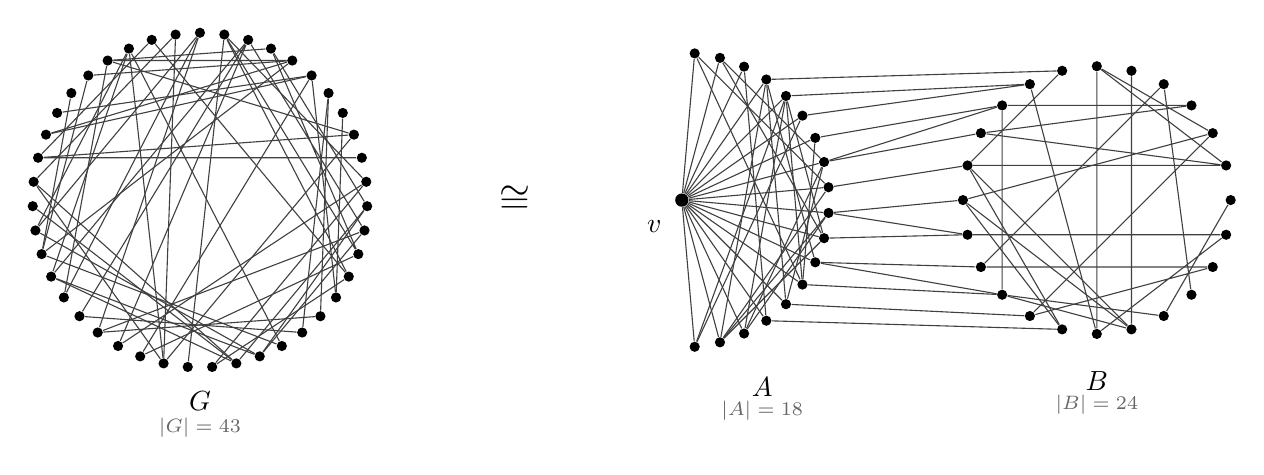
\begin{tikzpicture}[scale=0.85,
			vertex/.style={circle, fill, inner sep=1.3pt},
			pivot/.style={circle, fill, inner sep=1.7pt},
			e/.style={thin, black!75}
		]
		% Pivot vertex.
		\node[pivot, label={[label distance=1mm]below left:$v$}] (v) at (0,0) {};

		% Neighborhood A: 18 vertices, all adjacent to v.
		\foreach \i in {0,...,17} {
				\node[vertex] (a\i) at ({-85 + 10*\i}:2.2) {};
			}

		% Anti-neighborhood B: 24 vertices, none adjacent to v.
		\foreach \i [evaluate=\i as \bx using 6.2 + 2*cos(15*\i),
			evaluate=\i as \by using 2*sin(15*\i)] in {0,...,23} {
				\node[vertex] (b\i) at (\bx, \by) {};
			}

		% The whole graph G: 43 vertices on a circle.
		\foreach \i [evaluate=\i as \gx using -7.2 + 2.5*cos(90 + 8.372093*\i),
			evaluate=\i as \gy using 2.5*sin(90 + 8.372093*\i)] in {0,...,42} {
				\node[vertex] (g\i) at (\gx, \gy) {};
			}

		% Illustrative random edges inside G.
		\draw[e] (g13) -- (g39) (g16) -- (g41) (g18) -- (g41);
		\draw[e] (g1) -- (g10) (g32) -- (g40) (g10) -- (g23);
		\draw[e] (g3) -- (g25) (g9) -- (g34) (g29) -- (g42);
		\draw[e] (g18) -- (g33) (g19) -- (g38) (g0) -- (g12);
		\draw[e] (g20) -- (g35) (g33) -- (g42) (g1) -- (g20);
		\draw[e] (g30) -- (g40) (g30) -- (g42) (g31) -- (g41);
		\draw[e] (g0) -- (g17) (g21) -- (g42) (g7) -- (g38);
		\draw[e] (g14) -- (g24) (g8) -- (g39) (g5) -- (g13);
		\draw[e] (g4) -- (g39) (g22) -- (g33) (g0) -- (g15);
		\draw[e] (g24) -- (g32) (g10) -- (g20) (g3) -- (g20);
		\draw[e] (g14) -- (g23) (g19) -- (g30) (g3) -- (g12);
		\draw[e] (g12) -- (g24) (g17) -- (g27) (g28) -- (g38);
		\draw[e] (g17) -- (g31) (g4) -- (g40) (g3) -- (g14);
		\draw[e] (g13) -- (g25) (g4) -- (g15) (g9) -- (g35);
		\draw[e] (g8) -- (g38) (g23) -- (g32) (g24) -- (g31);
		\draw[e] (g5) -- (g39) (g6) -- (g13) (g27) -- (g37);
		\draw[e] (g22) -- (g29) (g14) -- (g41) (g11) -- (g23);
		\draw[e] (g16) -- (g26) (g2) -- (g29) (g2) -- (g9);
		\draw[e] (g28) -- (g36) (g26) -- (g37) (g4) -- (g35);

		% Edges from v into A.
		\foreach \i in {0,...,17} \draw[e] (v) -- (a\i);

		% Illustrative edges inside A.
		\draw[e] (a4) -- (a14) (a2) -- (a8) (a1) -- (a9);
		\draw[e] (a1) -- (a7) (a2) -- (a13) (a5) -- (a11);
		\draw[e] (a0) -- (a12) (a1) -- (a8) (a4) -- (a10);
		\draw[e] (a1) -- (a14) (a6) -- (a14) (a3) -- (a15);
		\draw[e] (a5) -- (a13) (a2) -- (a10) (a9) -- (a17);
		\draw[e] (a5) -- (a17) (a10) -- (a16) (a7) -- (a16);
		\draw[e] (a0) -- (a13) (a7) -- (a13);

		% Illustrative edges inside B.
		\draw[e] (b6) -- (b18) (b4) -- (b14) (b12) -- (b19);
		\draw[e] (b13) -- (b23) (b15) -- (b19) (b5) -- (b19);
		\draw[e] (b0) -- (b20) (b18) -- (b23) (b16) -- (b22);
		\draw[e] (b1) -- (b6) (b15) -- (b20) (b3) -- (b9);
		\draw[e] (b11) -- (b19) (b1) -- (b11) (b1) -- (b10);
		\draw[e] (b2) -- (b6) (b11) -- (b17) (b3) -- (b10);
		\draw[e] (b2) -- (b12) (b2) -- (b16) (b4) -- (b21);
		\draw[e] (b7) -- (b11) (b8) -- (b18) (b9) -- (b15);
		\draw[e] (b12) -- (b17) (b14) -- (b22);

		% Illustrative cross edges between A and B.
		\draw[e] (a8) -- (b12) (a9) -- (b11) (a7) -- (b13)
		(a10) -- (b10) (a6) -- (b14) (a11) -- (b9) (a5) -- (b15);
		\draw[e] (a3) -- (b17) (a4) -- (b16) (a6) -- (b15)
		(a8) -- (b13) (a10) -- (b9) (a12) -- (b8)
		(a13) -- (b8) (a14) -- (b7);

		% Isomorphism between the two depictions.
		\node[font=\Large] at (-2.5, 0) {$\cong$};

		% Group labels.
		\node at (-7.2, -3.0) {$G$};
		\node[font=\scriptsize, text=black!60] at (-7.2, -3.4) {$|G| = 43$};
		\node at (1.2, -2.8) {$A$};
		\node[font=\scriptsize, text=black!60] at (1.2, -3.15) {$|A| = 18$};
		\node at (6.2, -2.7) {$B$};
		\node[font=\scriptsize, text=black!60] at (6.2, -3.05) {$|B| = 24$};
	\end{tikzpicture}
	\caption{Illustrative decomposition into pivot $v$, neighborhood $A$ and anti-neighborhood $B$.}
\end{figure}
.

\begin{figure}[ht]
	\centering
	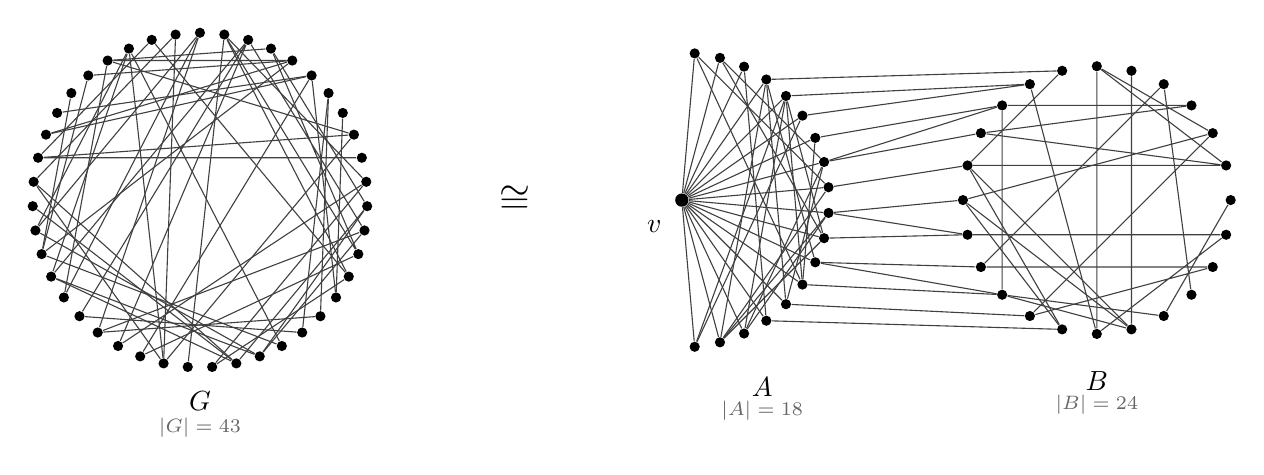
\begin{tikzpicture}[scale=0.85,
			vertex/.style={circle, fill, inner sep=1.3pt},
			pivot/.style={circle, fill, inner sep=1.7pt},
			e/.style={thin, black!75}
		]
		% Pivot vertex.
		\node[pivot, label={[label distance=1mm]below left:$v$}] (v) at (0,0) {};

		% Neighborhood A: 18 vertices, all adjacent to v.
		\foreach \i in {0,...,17} {
				\node[vertex] (a\i) at ({-85 + 10*\i}:2.2) {};
			}

		% Anti-neighborhood B: 24 vertices, none adjacent to v.
		\foreach \i [evaluate=\i as \bx using 6.2 + 2*cos(15*\i),
			evaluate=\i as \by using 2*sin(15*\i)] in {0,...,23} {
				\node[vertex] (b\i) at (\bx, \by) {};
			}

		% The whole graph G: 43 vertices on a circle.
		\foreach \i [evaluate=\i as \gx using -7.2 + 2.5*cos(90 + 8.372093*\i),
			evaluate=\i as \gy using 2.5*sin(90 + 8.372093*\i)] in {0,...,42} {
				\node[vertex] (g\i) at (\gx, \gy) {};
			}

		% Illustrative random edges inside G.
		\draw[e] (g13) -- (g39) (g16) -- (g41) (g18) -- (g41);
		\draw[e] (g1) -- (g10) (g32) -- (g40) (g10) -- (g23);
		\draw[e] (g3) -- (g25) (g9) -- (g34) (g29) -- (g42);
		\draw[e] (g18) -- (g33) (g19) -- (g38) (g0) -- (g12);
		\draw[e] (g20) -- (g35) (g33) -- (g42) (g1) -- (g20);
		\draw[e] (g30) -- (g40) (g30) -- (g42) (g31) -- (g41);
		\draw[e] (g0) -- (g17) (g21) -- (g42) (g7) -- (g38);
		\draw[e] (g14) -- (g24) (g8) -- (g39) (g5) -- (g13);
		\draw[e] (g4) -- (g39) (g22) -- (g33) (g0) -- (g15);
		\draw[e] (g24) -- (g32) (g10) -- (g20) (g3) -- (g20);
		\draw[e] (g14) -- (g23) (g19) -- (g30) (g3) -- (g12);
		\draw[e] (g12) -- (g24) (g17) -- (g27) (g28) -- (g38);
		\draw[e] (g17) -- (g31) (g4) -- (g40) (g3) -- (g14);
		\draw[e] (g13) -- (g25) (g4) -- (g15) (g9) -- (g35);
		\draw[e] (g8) -- (g38) (g23) -- (g32) (g24) -- (g31);
		\draw[e] (g5) -- (g39) (g6) -- (g13) (g27) -- (g37);
		\draw[e] (g22) -- (g29) (g14) -- (g41) (g11) -- (g23);
		\draw[e] (g16) -- (g26) (g2) -- (g29) (g2) -- (g9);
		\draw[e] (g28) -- (g36) (g26) -- (g37) (g4) -- (g35);

		% Edges from v into A.
		\foreach \i in {0,...,17} \draw[e] (v) -- (a\i);

		% Illustrative edges inside A.
		\draw[e] (a4) -- (a14) (a2) -- (a8) (a1) -- (a9);
		\draw[e] (a1) -- (a7) (a2) -- (a13) (a5) -- (a11);
		\draw[e] (a0) -- (a12) (a1) -- (a8) (a4) -- (a10);
		\draw[e] (a1) -- (a14) (a6) -- (a14) (a3) -- (a15);
		\draw[e] (a5) -- (a13) (a2) -- (a10) (a9) -- (a17);
		\draw[e] (a5) -- (a17) (a10) -- (a16) (a7) -- (a16);
		\draw[e] (a0) -- (a13) (a7) -- (a13);

		% Illustrative edges inside B.
		\draw[e] (b6) -- (b18) (b4) -- (b14) (b12) -- (b19);
		\draw[e] (b13) -- (b23) (b15) -- (b19) (b5) -- (b19);
		\draw[e] (b0) -- (b20) (b18) -- (b23) (b16) -- (b22);
		\draw[e] (b1) -- (b6) (b15) -- (b20) (b3) -- (b9);
		\draw[e] (b11) -- (b19) (b1) -- (b11) (b1) -- (b10);
		\draw[e] (b2) -- (b6) (b11) -- (b17) (b3) -- (b10);
		\draw[e] (b2) -- (b12) (b2) -- (b16) (b4) -- (b21);
		\draw[e] (b7) -- (b11) (b8) -- (b18) (b9) -- (b15);
		\draw[e] (b12) -- (b17) (b14) -- (b22);

		% Illustrative cross edges between A and B.
		\draw[e] (a8) -- (b12) (a9) -- (b11) (a7) -- (b13)
		(a10) -- (b10) (a6) -- (b14) (a11) -- (b9) (a5) -- (b15);
		\draw[e] (a3) -- (b17) (a4) -- (b16) (a6) -- (b15)
		(a8) -- (b13) (a10) -- (b9) (a12) -- (b8)
		(a13) -- (b8) (a14) -- (b7);

		% Isomorphism between the two depictions.
		\node[font=\Large] at (-2.5, 0) {$\cong$};

		% Group labels.
		\node at (-7.2, -3.0) {$G$};
		\node[font=\scriptsize, text=black!60] at (-7.2, -3.4) {$|G| = 43$};
		\node at (1.2, -2.8) {$A$};
		\node[font=\scriptsize, text=black!60] at (1.2, -3.15) {$|A| = 18$};
		\node at (6.2, -2.7) {$B$};
		\node[font=\scriptsize, text=black!60] at (6.2, -3.05) {$|B| = 24$};
	\end{tikzpicture}
	\caption{Illustrative decomposition into pivot $v$, neighborhood $A$ and anti-neighborhood $B$.}
\end{figure}
